\def\duedate{\today}
\def\HWnum{4}
\documentclass[10pt,a4paper]{book}

% custom section formatting
\usepackage{titlesec}
\titleformat{\chapter}[display]
{\normalfont\Large\filcenter\sffamily}
{\titlerule[1pt]%
\vspace{1pt}%
\titlerule
\vspace{1pc}%
\LARGE\MakeUppercase{\chaptertitlename} \thechapter}
{1pc}
{\titlerule
\vspace{1pc}%
\Huge}

% appendix handling
\usepackage[toc,page]{appendix}
    
% encoding for file and font
\usepackage[utf8]{inputenc}
\usepackage[T1]{fontenc}

% math formatting/tools
\usepackage{amsmath}
\usepackage{amssymb}
\usepackage{mathtools}
\usepackage[arrowdel]{physics}

% unit formatting
\usepackage{siunitx}
\AtBeginDocument{\RenewCommandCopy\qty\SI}

% figure formatting/tools
\usepackage{graphicx}
\usepackage{float}
\usepackage{subcaption}
\usepackage{multirow}
\usepackage{import}
\usepackage{pdfpages}
\usepackage{transparent}
\usepackage{currfile}

\NewDocumentCommand\incfig{O{1} m}{
    \def\svgwidth{#1\textwidth}
    \import{./Figures/\currfiledir}{#2.pdf_tex}
}

\newcommand{\bef}{\begin{figure}[h!tb]\centering}
\newcommand{\eef}{\end{figure}}

\newcommand{\bet}{\begin{table}[h!tb]\centering}
\newcommand{\eet}{\end{table}}

% hyperlink references 
\usepackage{hyperref}
\hypersetup{
    colorlinks=true,
    linkcolor=blue,
    filecolor=magenta,
    urlcolor=cyan,
    pdftitle={Physics 1 Notes},
    pdfauthor={Richard Whitehill},
    pdfpagemode=FullScreen
}
\urlstyle{same}

\newcommand{\eref}[1]{Eq.~(\ref{eq:#1})}
\newcommand{\erefs}[2]{Eqs.~(\ref{eq:#1})--(\ref{eq:#2})}

\newcommand{\fref}[1]{Fig.~(\ref{fig:#1})}
\newcommand{\frefs}[2]{Fig.~(\ref{fig:#1})--(\ref{fig:#2})}

\newcommand{\aref}[1]{Appendix~(\ref{app:#1})}
\newcommand{\sref}[1]{Section~(\ref{sec:#1})}
\newcommand{\srefs}[2]{Sections~(\ref{sec:#1})-(\ref{sec:#2})}

\newcommand{\tref}[1]{Table~(\ref{tab:#1})}
\newcommand{\trefs}[2]{Table~(\ref{tab:#1})--(\ref{tab:#2})}

% tcolorbox formatting/definitions
\usepackage[most]{tcolorbox}
\usepackage{xcolor}
\usepackage{xifthen}
\usepackage{parskip}

\definecolor{peach}{rgb}{1.0,0.8,0.64}

\DeclareTColorBox[auto counter, number within=chapter]{defbox}{O{}}{
    enhanced,
    boxrule=0pt,
    frame hidden,
    borderline west={4pt}{0pt}{green!50!black},
    colback=green!5,
    before upper=\textbf{Definition \thetcbcounter \ifthenelse{\isempty{#1}}{}{: #1} \\ },
    sharp corners
}

\newcommand*{\eqbox}{\tcboxmath[
    enhanced,
    colback=black!10!white,
    colframe=black,
    sharp corners,
    size=fbox,
    boxsep=8pt,
    boxrule=1pt
]}

\newtcolorbox[auto counter, number within=chapter]{exbox}{
    parbox=false,
    breakable,
    enhanced,
    sharp corners,
    boxrule=1pt,
    colback=white,
    colframe=black,
    before upper= \textbf{Example \thetcbcounter:}\,,
    before lower= \textbf{Solution:}\,,
    segmentation hidden
}

\newtcolorbox{resbox}{
    enhanced,
    colback=black!10!white,
    colframe=black,
    boxrule=1pt,
    boxsep=0pt,
    top=2pt,
    ams nodisplayskip,
    sharp corners
}


\begin{document}

\prob{1 -- Chapter 4 \# 7}{

Consider the one-dimensional problem of mass $m$ under the influence of a potential
\begin{eqnarray}
   V(x) = \begin{cases}
       -V_0 \delta(x) & |x| < a/2 \\
       \infty & |x| > a/2
   ,\end{cases}
\end{eqnarray}
where $V_0 > 0$. \\[1pt]

(a) Assume the particle's energy $E < 0$.
Show that there is a bound-state if a certain condition is satisfied.

(b) Assume the particle's energy $E > 0$.
Find the bound state energies in this case (a graphical solution of the relevant condition suffices).

(c) Compare the bound-state energies found in (b) above with those obtained in the infinitely deep well with $V(x) = 0$ if $|x| < a/2$ and $V(x) = \infty$ otherwise.
Comment the results.

}

\sol{

(a) For $E < 0$, the S.E. reads
\begin{eqnarray}
    \psi''(x) = - [v_0 \delta(x) - |\epsilon|] \psi(x)
,\end{eqnarray}
where $v_0 = 2 m V_0 / \hbar^2$ and $\epsilon = 2mE/\hbar^2 < 0$.
This has solution
\begin{eqnarray}
   \psi(x) = \begin{cases}
       A \cosh{(\kappa x)} + B \sinh{(\kappa x)} & x < 0 \\
       C \cosh{(\kappa x)} + D \sinh{(\kappa x)} & x > 0
   .\end{cases}
\end{eqnarray}
Note that it is implicitly understood that the interval of consideration is $|x| < a/2$ since $\psi \equiv 0$ for $|x| > a/2$.
The constants $A,~B,~C,~D$ are determined by normalization and the following boundary conditions (BCs):
\begin{align}
    \psi(-a/2) = 0 &\Rightarrow  A \cosh(-\kappa a/2) + B \sinh(-\kappa a/2) = 0 \\
    \psi(a/2) = 0 &\Rightarrow C \cosh(\kappa a/2) + D \sinh(\kappa a/2) = 0 \\
    \psi(0^{-}) = \psi(0^{+}) &\Rightarrow A = C \\
    \psi'(0^{+}) - \psi'(0^{-}) = -v_0 \psi(0) &\Rightarrow D \kappa - B \kappa = -v_0 A
.\end{align}
We can rearrange these equations to appear as (using $A = C$ to reduce the dimensionality of the problem)
\begin{eqnarray}
\begin{cases}
    A \cosh(\kappa a/2) - B \sinh(\kappa a/2) = 0 \\
    A \cosh(\kappa a/2) + D \sinh(\kappa a/2) = 0 \\
    Av_0 - B \kappa + D \kappa = 0
.\end{cases}
\end{eqnarray}
Observe that the first two equations tell us that $D = -B$, which means that we have the following $2 \times 2$ linear system
\begin{eqnarray}
\begin{cases}
    A \cosh(\kappa a/2) - B \sinh(\kappa a/2) = 0 \\
    A v_0 - 2\kappa B = 0
.\end{cases}
\end{eqnarray}
In order to have a non-trivial solution for the constants, we must have
\begin{gather}
   \det\begin{pmatrix}
       \cosh(\kappa a/2) & -\sinh(\kappa a /2) \\
       v_0 & -2 \kappa
   \end{pmatrix}
   = -2 \kappa \cosh(\frac{\kappa a}{2}) + v_0 \sinh(\frac{\kappa a}{2}) = 0
.\end{gather}
This gives the following condition on the bound state energy:
\begin{eqnarray}
    \tanh(\frac{z}{2}) = \frac{2 z}{z_0}
.\end{eqnarray}
Observe that the l.h.s and r.h.s. are monotonically increasing functions in $z$.
The derivative of the l.h.s, though is a strictly decreasing function of $z$, and furthermore, they intersect at $z = 0$ (which corresponds to $E = 0$ but our domain of interest is $z > 0$).
Hence, for a solution in the region $z > 0$ (there can be at most one) and therefore the existence of a bound state we must have
\begin{eqnarray}
    \dv{z} \tanh(\frac{z}{2})\Big|_{z = 0} = \frac{1}{2} > \frac{2}{z_0} \Rightarrow \eqbox{ z_0 > 4 }
.\end{eqnarray}

(b) For $E > 0$, the S.E. reads
\begin{eqnarray}
    \psi''(x) = -[ v_0 \delta(x) + \epsilon ] \psi(x)
.\end{eqnarray}
We then have the solution
\begin{eqnarray}
   \psi(x) = \begin{cases}
       A \cos(k x) + B \sin(kx) & x < 0 \\
       C \cos(kx) + D \sin(kx) & x > 0
   ,\end{cases}
\end{eqnarray}
where $k = \sqrt{\epsilon}$.
The boundary conditions are the same as above, which gives
\begin{gather}
\begin{cases}
    A \cos(ka/2) - B \sin(ka/2) = 0 \\
    C \cos(ka/2) + D \sin(ka/2) = 0 \\
    A = C \\
    D k - B k = -v_0 A
.\end{cases}
\end{gather}
Again, we have the third equality between $A$ and $C$ and $(D + B)\sin(ka/2) = 0$.
Notice from this we have two possible paths\footnote{In the previous part, we had $(D + B)\sinh(\kappa a/2) = 0$, which only admits $D = -B$ since $\sinh(x) = 0$ only if $x = 0$, which corresponds to $E = 0$.}.
First, we can have
\begin{eqnarray}
    \eqbox{ \sin(k a/2) = 0 \Rightarrow k = \frac{(2n) \pi}{a} }
,\end{eqnarray}
where $n = 1,2,\ldots$ (not $n=0$, though, so our wavefunction is non-trivial and indeed a bound state).
Interestingly, these are also the even bound state energies for the infinite square well.

On, the other hand, we can also have $D = -B$, which reduces the system to
\begin{eqnarray}
\label{eq:odd-bs-sys}
\begin{cases}
    A \cos(k a /2) - B \sin(k a/2) = 0 \\
    A v_0 - 2kB = 0
,\end{cases}
\end{eqnarray}
and gives us the following transcendental equation for the bound state energies: 
\begin{eqnarray}
    \label{eq:bound-state-cond}
    \eqbox{ \tan(\frac{z}{2}) = \frac{2z}{z_0} }
,\end{eqnarray}
where $z = ka$ and $z_0 = v_0 a$.

Observe that this condition admits an infinite set of discrete solutions $z$ for a given $z_0$ since $\tan(z/2)$ is $2\pi$-periodic, and hence, even if there is no solution for $0 < z < 2 \pi$, there will be for $z > 2\pi$\footnote{There is a solution on $0 < z < 2\pi$ for $z_0 < 4$.}.
Since this is a transcendental equation in terms of $z$, there is no closed form solution for $z$, and a numerical or approximate solution becomes necessary.
A graphical depiction of the bound state energies (as given by \eref{bound-state-cond}) is shown in \fref{prob1b}.

\begin{figure}[h!]
    \centering
    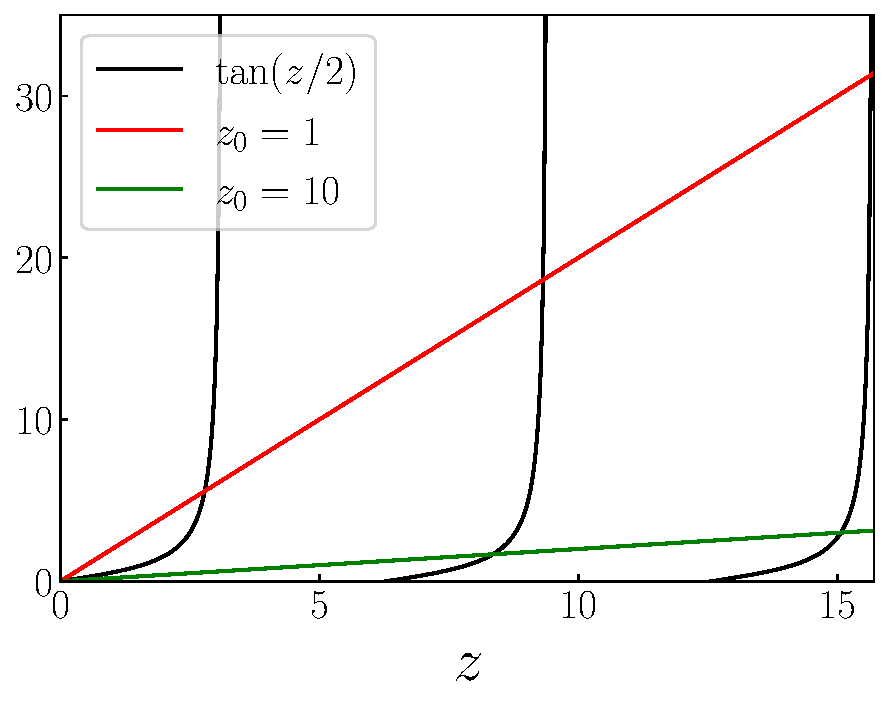
\includegraphics[width=0.5\textwidth]{prob1b.pdf}
    \caption{Plot of left and right sides of \eref{bound-state-cond} for two values of $z_0$. Note that where the black and red/green curves intersect give the bound state energies for a given $z_0$.}
    \label{fig:prob1b}
\end{figure}

(c) We obtain the bound-state energies of the infinitely deep well by taking $V_0 \rightarrow 0$.
The first case we analyzed are already equivalent to the even solutions of the infinite square well, so there is not work to be done there.

Next, from the r.h.s. of \eref{bound-state-cond} we find
\begin{eqnarray}
    \tan(\frac{z}{2}) \rightarrow \infty
.\end{eqnarray}
This happens when $z = \sqrt{\epsilon} a = (2n +1) \pi$ for $n = 0,1,\ldots$ or
\begin{eqnarray}
    \eqbox{ E_{n} = \frac{\hbar^2 \pi^2 (2n+1)^2 }{2 m a^2} }
,\end{eqnarray}
which gives us the odd energies of the infinite square well.
Furthermore, notice that the boundary conditions at $x = 0$ give $B = D$, which gives an odd wave function, coupled with $A = C$.


}


\prob{2 -- Chapter 5 \# 3}{

Calculate the transmission probability for a particle in a potential given by $V(x) = 0$ for $x < 0$ and $x > a$, and equal to a constant $V_0 > 0$ for $0 < x < a$.
Consider the two cases $0 < E < V_0$ and $E > V_0$.
Discuss the motion of a classical particle in the two cases. \\[1pt]

By introducing wave packets, calculate the transit time -- the time needed to traverse the barrier -- or the transmitted wave for the two cases $0 < E < V_0$ and $E > V_0$ and compare it to that of the classical particle.

}

\sol{

\textbf{Case 1:} $0 < E < V_0$ --
In this case we have wave functions
\begin{align}
    \psi^{(1)}(x) &= \begin{cases}
       A e^{i k x} + B e^{-ikx} & x < 0 \\
       C e^{\kappa x} + D e^{-\kappa x} & 0 < x < a \\
       E e^{i k x} & x > a
   ,\end{cases} \\
        \psi^{(2)}(x) &= \begin{cases}
            A e^{-ikx} & x < 0 \\
            B e^{\kappa x} + C e^{-\kappa x} & 0 < x < a \\
            D e^{ikx} + E e^{-ikx} & x > a
        \end{cases}
\end{align}
where $k = \sqrt{\epsilon}$ ($\epsilon = 2mE/\hbar^2$) and $\kappa = \sqrt{v_0 - \epsilon}$ ($v_0 = 2mV_0/\hbar^2$).
Observe that by choosing these solutions as our linearly independent set, we can consider $\psi^{(1)}$ alone to calculate the transmission and reflection probabilities, and the results will apply for $\psi^{(2)}$.
This is seen by noticing that relecting $\psi^{(2)}$ about $x = a/2$ gives $\psi^{(1)}$.

Digressing, the setup imposes the boundary conditions
\begin{align}
    \psi(0^{+}) = \psi(0^{-}) &\Rightarrow A + B = C + D \\
    \psi'(0^{+}) = \psi'(0^{-}) &\Rightarrow ik(A - B) = \kappa (C - D) \\
    \psi(a^{+}) = \psi(a^{-}) &\Rightarrow E e^{ika} = Ce^{\kappa a} + De^{-\kappa a} \\
    \psi'(a^{+}) = \psi'(a^{-}) &\Rightarrow ik E e^{ika} = \kappa (Ce^{\kappa a} - De^{-\kappa a})
.\end{align}
Notice that we have four equations for five unknowns, so we will let $A$ be our undetermined parameter and solve for $B$ and $E$ in terms of $A$\footnote{I have delegated this task to the \textit{sympy} package from \textit{python} since it is more efficient at these kinds of things.}:
\begin{align}
    \frac{B}{A} &= \frac{(\kappa^2 + k^2)(e^{2\kappa a} - 1)}{[k(e^{\kappa a} + 1) + i\kappa (e^{\kappa a} - 1)][k(e^{\kappa a} - 1) + i\kappa (e^{\kappa a} + 1)]} \\
    \frac{E}{A} &= \frac{4 i \kappa k e^{\kappa a} e^{-ika}}{[k(e^{\kappa a} + 1) + i\kappa (e^{\kappa a} - 1)][k(e^{\kappa a} - 1) + i\kappa (e^{\kappa a} + 1)]}
.\end{align}
From this, we get the transmission coefficient
\begin{eqnarray}
    \begin{aligned}
        T = \Big| \frac{E}{A} \Big|^2 &= \frac{16 \kappa^2 k^2 e^{2 \kappa a}}{[k^2(e^{\kappa a} + 1)^2 + \kappa^2(e^{\kappa a} - 1)^2][k^2(e^{\kappa a} - 1)^2 + \kappa^2(e^{\kappa a} + 1)^2]} \\
                                      &= \frac{\kappa^2 k^2}{[k^2 \cosh^2(\kappa a/2) + \kappa^2 \sinh^2(\kappa a/2)][k^2 \sinh^2(\kappa a/2) + \kappa^2 \cosh^2(\kappa a/2)]} \\
                                      &= \frac{8 \kappa^2 k^2}{[ (\kappa^2 + k^2)^2 \cosh(2 \kappa a) - (\kappa^{4} - 6 \kappa^2 k^2 + k^{4}) ]} \\
                                      &= \eqbox{ \frac{4 \kappa^2 k^2}{(k^2 + \kappa^2)^2 \cosh^2(\kappa a) - (k^2 - \kappa^2)^2} = \frac{4 \epsilon (v_0 - \epsilon)}{4 \epsilon (v_0 - \epsilon) + v_0^2 \sinh^2(\sqrt{v_0 - \epsilon} a)} }
    .\end{aligned}
\end{eqnarray}

Let us introduce a wave packet here as follows\footnote{We absorb the conventional $1/\sqrt{2\pi}$ factor into the profile function $g(k)$ to make the expressions a bit more digestible.}:
\begin{eqnarray}
    \Psi(x,t) = \int_{0}^{k_0} \dd{k} g(k) \psi_{k}^{(1)}(x) e^{-i \omega t}
\end{eqnarray}
where $g(k)$ is strongly localized around some $k_{\star}$ and $\omega = \hbar k^2/2m$.
We expect that the time for the particle to ``tunnel'' through the barrier will manifest itself as a kind of time-delay in the transmitted wave packet
\begin{eqnarray}
    \label{eq:T-wave-packet}
    \Psi_{T}(x,t) = \int \dd{k} g(k) |e(k)| e^{i[k(x-a) - \omega t + \delta(k)]}
,\end{eqnarray}
where $\tan{\delta(k)} = \Im[e(k)]/\Re[e(k)]$.
We use the stationary phase method to approximate this integral, defining $\varphi(k) = k(x-a) - \omega(k) t + \delta(k)$, and $x_{T}$ is defined such that $\varphi'(k_{\star};x=x_{T}) = (x_{T} - a) - \omega'(k_{\star}) t + \delta'(k_{\star}) = 0$.
Rewriting a bit, we have
\begin{eqnarray}
    x_{T} - a = \omega'(k_{\star})t - \delta'(k_{\star}) = \frac{\hbar k_{\star}}{m} \Big[ t - \frac{m}{\hbar k_{\star}} \delta'(k_{\star}) \Big]
.\end{eqnarray}
Thus, \eref{T-wave-packet} becomes
\begin{eqnarray}
    \Psi_{T}(x,t) \approx |e(k_{\star})| e^{i(k_{\star} x - \omega_{\star} t + \delta(k_{\star}))} \int \dd{k} g(k) e^{i[x - x_{T}(t)][k-k_{\star}]}
.\end{eqnarray}
All that remains is to determine $\delta'(k_{\star})$ such that we can determine the time delay for a particle to traverse the potential step.
Defining
\begin{eqnarray}
    e(k) = \frac{E}{A} e^{ika} = \frac{i \kappa k}{[k \cosh(\kappa a/2) + i\kappa \sinh(\kappa a/2)][k \sinh(\kappa a/2) + i\kappa \cosh(\kappa a/2)]}
.\end{eqnarray}
For our analysis, we only care about the phase of $e(k)$, and for a complex number $z = v/w = w^{*} v/|w|^2$, $\arg{z} = \arctan[\Im(w^{*}v)/\Re(w^{*}v)]$.
We define
\begin{eqnarray}
    \begin{aligned}
        z &= i \kappa k [k \cosh(\kappa a/2) - i\kappa \sinh(\kappa a/2)][k \sinh(\kappa a/2) - i\kappa \cosh(\kappa a/2)] \\
          &= \kappa k \Big( \kappa k \cosh(\kappa a) - i \frac{(\kappa^2 - k^2)}{2} \sinh(\kappa a) \Big)
    \end{aligned}
,\end{eqnarray}
and
\begin{eqnarray}
    \delta(k) = \arctan(\frac{\Im(z)}{\Re(z)}) = - \arctan\Bigg[ \frac{\kappa^2 - k^2}{2 \kappa k} \tanh(\kappa a) \Bigg]
.\end{eqnarray}
Thus,
\begin{eqnarray}
    \begin{aligned}
        \delta'(k) &= -\frac{4 \kappa^2 k^2}{4 \kappa^2 k^2 + (\kappa^2 - k^2)^2\tanh^2(\kappa a)} \Bigg\{ \tanh(\kappa a) \dv{k} \Big( \frac{\kappa^2 - k^2}{2 \kappa k} \Big) + \frac{\kappa^2 - k^2}{2 \kappa k} \frac{a ~ {\rm d} \kappa / {\rm d} k}{\cosh^2(\kappa a)} \Bigg\} \\
                   &= \frac{4 \kappa^2 k^2}{4 \kappa^2 k^2 + (\kappa^2 - k^2)^2\tanh^2(\kappa a)} \Bigg\{ \tanh(\kappa a) \frac{(\kappa^2 + k^2)^2}{2 \kappa^3 k^2} + \frac{\kappa^2 - k^2}{2 \kappa k} \frac{a k}{\kappa \cosh^2(\kappa a)} \Bigg\} \\
                   &= \frac{4 \kappa^2 k^2}{4 \kappa^2 k^2 + (\kappa^2 - k^2)^2\tanh^2(\kappa a)} \Bigg\{ \tanh(\kappa a) \frac{(\kappa^2 + k^2)^2}{2 \kappa^3 k^2} + \frac{\kappa^2 - k^2}{2 \kappa^2} \frac{a}{\cosh^2(\kappa a)} \Bigg\} \\
                   &= \frac{2(\kappa^2 + k^2)^2}{\kappa [ 4 \kappa^2 k^2 + (\kappa^2 - k^2)^2 \tanh^2(\kappa a) ]} \Bigg\{ \tanh(\kappa a) + \frac{(\kappa^2 - k^2) k^2 \kappa a}{(\kappa^2 + k^2)^2 \cosh^2(\kappa a)} \Bigg\}
    .\end{aligned}
\end{eqnarray}


This case gives quite different results than the classical expectation, which is that the particle hits the potential wall and reflects back without fail.

\textbf{Case 2:} $E > V_0$ -- In this case, the two linearly independent wave functions can be written as
\begin{align}
    \psi^{(1)}(x) &= \begin{cases}
       A e^{i k x} + B e^{-ikx} & x < 0 \\
       C e^{i K x} + D e^{-i K x} & 0 < x < a \\
       E e^{i k x} & x > a
   ,\end{cases} \\
    \psi^{(2)}(x) &= \begin{cases}
        A e^{-ikx} & x < 0 \\
        B e^{i K x} + C e^{-i K x} & 0 < x < a \\
        D e^{ikx} + E e^{-ikx} & x > a
    ,\end{cases}
\end{align}
where $K = \sqrt{\epsilon - v_0}$.
The boundary conditions give
\begin{eqnarray}
\begin{cases}
    A + B = C + D \\
    k(A - B) = K (C - D) \\
    Ce^{i K a} + D e^{-i K a} = E e^{i k a} \\
    \tilde{k}( Ce^{i K a} - D e^{-i K a}) = k E e^{i k a}
,\end{cases}
\end{eqnarray}
and solving gives
\begin{eqnarray}
    \begin{aligned}
        \frac{E}{A} &= -\frac{4 K k e^{i(K - k)a}}{[K(e^{i K a} + 1) - k(e^{i K a} - 1)][K(e^{i K a} - 1) - k(e^{i K a} + 1)]} \\
                    &= -\frac{K k e^{-i k a}}{[K\cos{(K a/2)} - ik \sin{(K a /2)}][iK\sin{(K a/2)} - k\cos{(K a/2)}]}
    .\end{aligned}
\end{eqnarray}
Thus, the transmission probability is\footnote{After spending time doing all this algebra, it dawned on me that $K = i\kappa$, so I could have used the property $\cosh(iKa) = \cos(Ka)$ and saved a lot of work to get the same result!}
\begin{eqnarray}
    \begin{aligned}
        T = \Big| \frac{E}{A} \Big|^2 &= \frac{K^2 k^2}{[K^2 \cos^2(K a/2) + k^2 \sin^2(K a/2)][K^2 \sin^2(K a/2) + k^2 \cos^2(K a/2)]} \\
                                      &= \frac{4K^2 k^2}{(K^{4} + k^{4})(1 - \cos^2(Ka)) + 2K^2k^2(\cos^2(Ka) + 1)} \\
                                      &= \eqbox{ \frac{4 K^2 k^2}{(k^2 + K^2)^2 - (k^2 - K^2)^2\cos^2(Ka)} }
    .\end{aligned}
\end{eqnarray}

Using the replacement $\kappa \rightarrow i K$, we can quickly obtain the traversal time from
\begin{eqnarray}
    \delta'(k) = \frac{2(k^2 - K^2)^2}{K[-4K^2k^2 + (K^2 + k^2)^2 \tan^2(K a)]} \Bigg\{ \tan(Ka) - \frac{(K^2 + k^2) k^2 Ka}{(k^2 - K^2)^2 \cos^2(Ka)} \Bigg\}
.\end{eqnarray}


In the classical case, a particle of mass $m$ traverses the potential step every time with speed
\begin{eqnarray}
    v = \sqrt{2m(E - V_0)}
,\end{eqnarray}
which means it takes time
\begin{eqnarray}
   t = \frac{1}{a}\sqrt{2m(E - V_0)}
\end{eqnarray}
to traverse the potential step.

}


\prob{3 -- Chapter 5 \# 6}{

Consider the one-dimensional potential $V(x)$ given by
\begin{eqnarray}
   V(x < 0) = \infty, \quad V(0 < x < a) = -V_0, \quad V(x > a) = 0,
,\end{eqnarray}
with $V_0 > 0$. \\[1pt]

(a) Discuss the energy spectrum: for what energies (if any) are there bound states?
For what energies are there continuum states?
What is the degeneracy of the energy eigenvalues?

(b) Assume the energy $E$ of the particle is less than zero.
Determine under what conditions there is at least a bound state.

(c) Show that for $x > a$ the positive energy solution (up to an overall constant) can be written as
\begin{eqnarray}
    \psi(x) = e^{i[k(x - a) - 2 \delta]} + e^{-ik(x-a)}
.\end{eqnarray}
Determine $\delta$ and the solution $\psi(x)$ in $0 < x < a$ (up to the overall constant, of course).
Calculate the reflection coefficient.

(d) Denote with $\psi_{k}(x)$ the complete positive-energy solution obtained in part (c) above, and consider the wave packet
\begin{eqnarray}
    \Psi(x,t) = \int_{0}^{\infty} \dd{k} g(k) \psi_{k}(x) e^{-i \omega t} \quad {\rm with}~\omega = \frac{E}{\hbar} = \frac{\hbar k^2}{2m}
,\end{eqnarray}
where the real function $g(k)$ is sharply peaked at $k_0$.
Examine the incident and reflected wave packets in the region $x > a$, and show that the incident wave packet reaches the edge of the potential well at $x = a$ at time $t = 0$, while the reflected wave packet leaves this edge with a time delay $\tau$.
Calculate $\tau$ and show that it is given by
\begin{eqnarray}
    \tau = \frac{2 a m}{\hbar \sqrt{\epsilon_0}} \frac{1}{\epsilon_0 + v_0 \cos^2{(K_0 a)}} \Big[ \epsilon_0 + v_0 \frac{\sin{(2 K_0 a)}}{2 K_0 a} \Big]
,\end{eqnarray}
where $\epsilon_0 = k_0^2$ and $K_0 = \sqrt{k_0^2 + v_0}$.
Discuss the limit $\epsilon_0 \gg v_0$.
Under what conditions will $\tau$ be very long?
Explain.

}

\sol{

(a) Bound states (no degeneracy) may arise for $-V_0 < E < 0$, while continuum states arise for $E > 0$.
For the continuum states, there is no degeneracy in the energy spectrum.
When one writes the solution for $\psi$ in the region $x > 0$, there are four undetermined constants.
There are three constraints on these from boundary conditions (we cannot impose normalization on the bare continuum states), which leaves only one undetermined constant and hence only one solution (up to a constant) for a given energy.

%Note that $E = 0$ is not a valid energy for a physical system since this gives $\psi \equiv 0$ for all $x$.

(b) For the bound states, we have 
\begin{eqnarray}
   \psi(x) = \begin{cases}
       0 & x < 0 \\
       A \sin(Kx) & 0 < x < a \\
       B e^{-\kappa(x - a)} & x > a
   ,\end{cases}
\end{eqnarray}
where $K = \sqrt{v_0 - |\epsilon|}$ and $\kappa = \sqrt{|\epsilon|}$.
Note that we have thrown away the $\cos(Kx)$ solution in the region $0 < x < a$ by using $\psi(0) = 0$.
We then have
\begin{eqnarray}
    \begin{cases}
    A \sin(Ka) = B \\
    KA\cos(Ka) = -\kappa B
    ,\end{cases}
\end{eqnarray}
which must be linearly dependent and give bound state energies satisfying
\begin{eqnarray}
    \eqbox{ \tan(Ka) = -\frac{K}{\kappa} \Leftrightarrow \tan(\sqrt{v_0 - |\epsilon|} a) = - \sqrt{\frac{v_0}{|\epsilon|} - 1} }
.\end{eqnarray}

If we denote $z = Ka$ and $z_0^2 = v_0a^2$, then we have the equation
\begin{eqnarray}
    \label{eq:bs-cond-3b}
    \tan{z} = - \frac{z}{\sqrt{z_0^2 - z^2}}
.\end{eqnarray}
A plot in \fref{prob3b} shows these two curves for $z_0 = 6$.
Clearly, there are two solutions for $z$ in this case.
Note that $\tan{z}$ is defined on the entire real axis as a real function, but the r.h.s. is not. In fact, its domain is $(0,z_0)$, and it comes in with a negative sign.
Hence, $z_0 > \pi/2$ for the existence of one solution, and furthermore, if $z_0 > (N - 1/2) \pi$ for $N = 1,2,\ldots$, there are $N$ solutions.

\begin{figure}[h!]
    \centering
    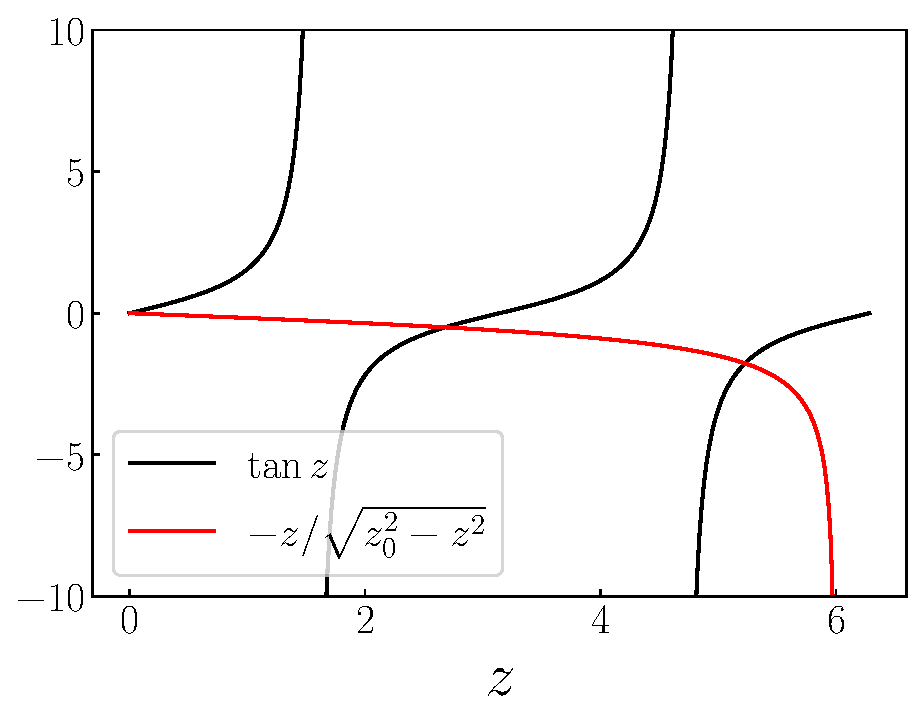
\includegraphics[width=0.5\textwidth]{prob3b.pdf}
    \caption{Plot of curves on the l.h.s. and r.h.s. of \eref{bs-cond-3b} for $z_0 = 6$.}
    \label{fig:prob3b}
\end{figure}

(c) If $E > 0$, then 
\begin{eqnarray}
   \psi(x) = \begin{cases}
       0 & x < 0 \\
       A \sin(Kx) & 0 < x < a \\
       B e^{i k (x-a)} + e^{-i k (x-a)} & x > a
   ,\end{cases}
\end{eqnarray}
Note that there is only one solution for each energy $\psi$.
The boundary conditions at $x = a$ give
\begin{eqnarray}
\begin{cases}
    A \sin(Ka) = B + 1 \\
    KA \cos(Ka) = ik(B - 1)
.\end{cases}
\end{eqnarray}
We then find
\begin{align}
    A &= \frac{2k}{k\sin(Ka) + iK \cos(Ka)} \\
    B &= \frac{\tan(Ka) - iK/k}{\tan(Ka) + iK/k}
.\end{align}
Notice that $|B| = 1$ and\footnote{We go from the first line to the second line by using $\tan(2x) = \tan{x}/(1 - \tan^2{x})$ and solving for $\tan^2{x}$.}
\begin{align}
    &\frac{\Im(B)}{\Re(B)} = \frac{2 K k \tan(Ka)}{k^2 \tan^2(Ka) - K^2} = \tan(2 \delta) \\
    &\Rightarrow \eqbox{ \tan \delta = -\frac{k}{K} \tan(Ka) }
.\end{align}
Hence, we can write
\begin{eqnarray}
    \eqbox{ \psi(x) = e^{i[k(x-a) - 2\delta]} + e^{-ik(x-a)} }
\end{eqnarray}
for $x > a$.

The reflection coefficient is defined as
\begin{eqnarray}
    R = |j_{r}|/|j_{i}| = \frac{\hbar k/m}{\hbar k/m} = 1
.\end{eqnarray}

(d) We introduce the wave packet 
\begin{eqnarray}
    \begin{aligned}
        \Psi(x,t) &= \int_{0}^{\infty} \dd{k} g(k) \psi_{k}(x) e^{-i \omega t} \\
                  &= \begin{cases}
                      0 & x < 0 \\
                      \int \dd{k} g(k) A(k) \sin(Kx) e^{-i \omega t} & 0 < x < a \\
                      \int \dd{k} g(k) e^{i[k(x-a) - \omega t - 2\delta(k)]} + \int \dd{k} g(k) e^{-i[k(x-a) + \omega t]} & x > a
                  \end{cases}
    .\end{aligned}
\end{eqnarray}
The reflected and incident wave packets are the first and second terms of the wave function in the region $x > a$.
First, we look at the incident wave packet:
\begin{eqnarray}
    \begin{aligned}
        \Psi_{I}(x,t) &= \int \dd{k} g(k) e^{-i[k(x-a) + \omega t]} \approx e^{-i[k_0(x-a) + \omega_0 t]} \int \dd{k} g(k) e^{-i[(x - a) + (\hbar k_0/m)t][k-k_0]} \\
                      &= e^{-i[k(x-a) + \omega_0 t]} \int \dd{k} g(k) e^{-i[x - x_{I}(t)][k-k_0]}
    ,\end{aligned}
\end{eqnarray}
where $x_{I}(t) - a = - (\hbar k_0/m)t$.

Now, we look at the reflected wave packet:
\begin{eqnarray}
    \Psi_{T}(x,t) \approx e^{i[k_0(x-a) - \omega_0 t - 2\delta(k_0)]} \int \dd{k} g(k) e^{i[x - x_{T}(t)][k-k_0]}
,\end{eqnarray}
where $x_{T}(t) - a = (\hbar k_0/m)t + 2\delta'(k_0) = (\hbar k_0/m)[t - \tau]$, where $\tau = -(2m/\hbar k_0) \delta'(k_0)$.
We now determine $\delta'(k_0)$:
\begin{eqnarray}
    \begin{aligned}
        \delta'(k) &= -\frac{1}{K^3} \Bigg[ (k^2 - K^2)\tan^2(Ka) - k^2 Ka \sec^2(Ka) \Bigg] \frac{K^2}{K^2 + k^2 \tan^2(Ka)} \\
                   &\Rightarrow \delta'(k_0) = -\frac{1}{K_0(K_0^2 + k^2 \tan^2(K_0a))}\Bigg[ (k_0^2 - K_0^2) \tan(K_0a) - \frac{k_0^2 K_0 a}{\cos^2(K_0a)} \Bigg] \\
                   &\phantom{\Rightarrow ~ \delta'(k_0)} = -\frac{2k_0^2 K_0 a + (K_0^2 - k_0^2) \sin(2K_0a)}{2K_0[k_0^2 + (K_0^2 - k_0^2)\cos^2(K_0a) ]}
    .\end{aligned}
\end{eqnarray}
Then
\begin{eqnarray}
    \eqbox{ \tau = \frac{2 m a}{\hbar \sqrt{\epsilon_0}} \frac{1}{\epsilon_0 + v_0 \cos^2(a \sqrt{v_0 + \epsilon_0})} \Bigg[ \epsilon_0 + \frac{v_0}{2 a \sqrt{\epsilon_0 + v_0}} \sin(2 a \sqrt{v_0 + \epsilon_0}) \Bigg] }
.\end{eqnarray}

If we consider $\epsilon_0 \gg v_0$, then
\begin{eqnarray}
    \eqbox{ \tau \approx \frac{2 m a}{\hbar \sqrt{\epsilon_0}} \Bigg[ 1 + \frac{v_0}{2a\epsilon_0\sqrt{\epsilon_0}} \sin(2a\sqrt{\epsilon_0}) \Bigg] \sim \frac{2ma}{\hbar \sqrt{\epsilon_0}} }
.\end{eqnarray}
Next, notice that $\tau$ is relatively large for $\epsilon_0 \rightarrow 0$ since
\begin{eqnarray}
   \tau \sim \frac{\tan(a\sqrt{v_0})}{a\sqrt{v_0}} \frac{1}{\sqrt{\epsilon}}
.\end{eqnarray}
Additionally, if $K_0 a = (n + 1/2) \pi$ for natural numbers $n$ such that $K_0 > \sqrt{v_0}$.
In this case $\sin(2K_0a) = 0$ and $\cos(K_0a) = 0$, meaning
\begin{eqnarray}
   \tau = \frac{2 m a}{\hbar \sqrt{\epsilon_n}} 
.\end{eqnarray}
For the lower lying energies given by the condition above, $\epsilon_{n}$ is relatively small, and $\tau_{n}$ is relatively large.


}


\prob{4 -- Chapter 5 \# 8}{

Consider a particle of mass $m$ confined in the region $x \geq 0$ and subject to a repulsive $\delta$-function potential located at $x = a$,
\begin{eqnarray}
    V(x) = \frac{\hbar^2}{2m} v_0 \delta(x - a) \quad {\rm for} ~ x \geq 0
.\end{eqnarray}

(a) Without doing any detailed calculations, explain why the reflection coefficient is unity in this case for any $\epsilon > 0$.

(b) Obtain the complete solution $\psi_{k}(x)$ with $k = \sqrt{\epsilon}$ in the whole allowed region $x \geq 0$, thus justifying the inference above.

(c) Construct the wave packet
\begin{eqnarray}
    \Psi(x,t) = \int_{0}^{\infty} \frac{\dd{k}}{\sqrt{2 \pi}} g(k) \psi_{k}(x) e^{-i \omega t} \quad \omega = \frac{\hbar k^2}{2m}
,\end{eqnarray}
where the profile function $g(k)$ is assumed to be real and strongly peaked at $k^{*} > 0$.
Show that the center of the incident wave packet reaches $a$ at time $t = 0$ and that the center of the reflected wave packet moves from $a$ back to infinity with a time delay $2 \tau$.
Determine $\tau$.

(d) Show that the magnitude squared of the wave packet in the region $0 < x < a$ is suppressed by the factor $1/\rho_{k}^2$.
Provide a plot of $1/\rho_{k}^2$ for $x_0 = v_0 a = 50$ as a function of $x = ka$ in the range $0 < x \leq 20$.
Comment on the figure.

(e) Compute the time delay $\tau$ and provide a plot of $\tau / \tau_0$, where $\tau_0 = ma^2/\hbar$, for the case $x_0 = 50$ and $x$ in the range 0-20, as above.
Comment on the figure.

}

\sol{

(a) It is simple to intuitively see why the reflection coefficient here is unity.
Let us imagine a wave packet representation for a particle in this potential.
Even if a particle is transmitted across the barrier at $x = a$, the infinite potential well will reflect the particle.
From then, there is a probability that either the particle will be transmitted back into the region $x > a$ or be relected back into $0 < x < a$.
In the former situation, the particle continues on to $x \rightarrow \infty$ without obstruction.
In the latter situation, we repeat the above logic until transmission eventually occurs at some $(N+1)^{\rm th}$ encounter with the barrier at $x = a$\footnote{Transmission back across the potential well must occur since if we send a particle towards the barrier at $x = a$ with the same energy a sufficient number of times, there will eventually be an event where transmission occurs by the law of large numbers. Otherwise the proability of transmission is zero, and there was no need to consider this case in the first place!}.
The transmission probability is related to the probability current density at times much after the interaction at $t = 0$.
For sufficiently large times, we would see that $j \equiv 0$ (that is, the amplitude of the wave function in the region $x < a$ goes to zero at sufficiently large times) in the region $x < a$, meaning that the particle has been reflected back to $x > a$.

(b) The Schr\"{o}dinger equation for this potential is
\begin{eqnarray}
    \psi''(x) = [v(x) - \epsilon] \psi(x) = [ v_0 \delta(x - a) - \epsilon ] \psi(x)
.\end{eqnarray}
Note that the first equality is valid for all $x$, while the second is only valid for $x > 0$.
Note that $\psi \equiv 0$ for $x < 0$, so the only interesting region is $x > 0$.

The S.E. has solution ($x > 0$)
\begin{eqnarray}
    \psi(x) = \begin{cases}
        A \sin(kx) & x < a \\
        B e^{ik(x-a)} + e^{-ik(x-a)} & x > a
    ,\end{cases}
\end{eqnarray}
where $k = \sqrt{\epsilon}$.
Note that we have already used the BC $\psi(x) = 0$ to rule out $\cos(kx)$ as a solution in the region $x < a$ and also that we have scaled the wave function (since it is not normalizable and hence only determined up to a constant) such that the term $e^{-ik(x-a)}$ only has the global undetermined constant in front of it.
We have two more BCs:
\begin{align}
    \psi(a^{+}) = \psi(a^{-}) &\Rightarrow A \sinh(ka) = B + 1 \\
    \psi'(a^{+}) - \psi'(a^{-}) = v_0 \psi(a) &\Rightarrow ik(B - 1) - kA\cosh(ka) = v_0 (B+1)
.\end{align}
Solving for $A$ and $B$, we find
\begin{align}
    A = \frac{2ik}{-[k \cos(ka) + v_0 \sin(ka)] + i k \sin(ka)} \\
    B = \frac{[k \cos(ka) + v_0 \sin(ka)) + i k \sin(ka)}{-[k\cos(ka) + v_0 \sin(ka)] + ik\sin(ka)}
.\end{align}

Observe from the solution to $A$ and $B$ here and the form of the wave function that the transmission coefficient
\begin{eqnarray}
    T = |j_{t}|/|j_{i}| = 0
,\end{eqnarray}
since $j_{t} = (\hbar/2mi)|A|^2 [ \sinh(kx) \cosh(kx) - {\rm c.c.}] = 0$, and therefore, $R = 1 - T = 1$, confirming our argument above.
Additionally, we could have done this directly as follows:
\begin{eqnarray}
    \eqbox{ R = |j_{r}| / |j_{i}| = \frac{\hbar k |B|^2/m}{\hbar k/m} = |B|^2 = 1 }
,\end{eqnarray}
since $B$ is of the form $-z/z^{*}$, meaning $|B|^2 = (-z/z^{*})(-z^{*}/z) = 1$.
Using this, we can write the wavefunction as
\begin{eqnarray}
    \psi(x) = \begin{cases}
        A(k) \sin(kx) \\
        e^{i[k(x-a) - 2\delta]} + e^{-ik(x-a)}
    ,\end{cases}
\end{eqnarray}
where
\begin{eqnarray}
    \delta = \arctan(\frac{k + v_0\tan(ka)}{k\tan(ka)})
.\end{eqnarray}

(c) We now construct a wave-packet as follows:
\begin{eqnarray}
    \begin{aligned}
        \Psi(x,t) &= \int_{0}^{\infty} \frac{\dd{k}}{\sqrt{2 \pi}} g(k) \psi_{k}(x) e^{-i \omega t} \\
                  &= \begin{cases}
                      \displaystyle \int \frac{\dd{k}}{\sqrt{2\pi}} g(k) A(k) \sin(ka) & x < a \\
                      \displaystyle \int \frac{\dd{k}}{\sqrt{2\pi}} g(k) e^{i[k(x-a) - \omega t - 2\delta]} + \int \frac{\dd{k}}{\sqrt{2 \pi}} g(k) e^{-i[k(x-a) + \omega t]} & x > a
                  .\end{cases}
    \end{aligned}
\end{eqnarray}
In this part, we are interested in the region $x > a$.
First, the incident wave-packet
\begin{eqnarray}
    \begin{aligned}
        \Psi_{I}(x,t) &= \int \frac{\dd{k}}{\sqrt{2 \pi}} e^{-i[k(x-a) + \omega t]} \\
                      &\approx e^{-i[k_{\star}(x-a) + \omega_{\star} t]} \int \frac{\dd{k}}{\sqrt{2\pi}} g(k) e^{-i[x-x_{I}(t)][k-k_{\star}]}
    ,\end{aligned}
\end{eqnarray}
where $x_{I}(t) - a = -(\hbar k / m) t$.
Notice that this tells us the center of the incident wave packet $x_{I} = a$ at $t = 0$.

Next, the reflected wave-packet:
\begin{eqnarray}
    \begin{aligned}
        \Psi_{R}(x,t) &= \int \frac{\dd{k}}{\sqrt{2\pi}} g(k) e^{i[k(x-a) - \omega t - 2\delta(k)]} \\
                      &\approx e^{i[k_{\star}(x-a) - \omega_{\star} t - 2\delta(k_{\star})]} \int \frac{\dd{k}}{\sqrt{2 \pi}} e^{i[x-x_{R}(t)][k - k_{\star}]}
    ,\end{aligned}
\end{eqnarray}
where $x_{R}(t) - a = (\hbar k_{\star}/m)t + 2\delta'(k_{\star}) = (\hbar k_{\star}/m)[t - 2\tau]$ and $\tau = -(m/\hbar k_{\star}) \delta'(k_{\star})$.
Hence, this wave-packet is at position $x_{R} = a$ at $t = 2\tau$, which we interpret as a kind of delay between incidence and reflection.
Evaluating $\delta'(k)$, we find
\begin{eqnarray}
    \delta'(k) = - \frac{k^2a + v_0\sin^2(ka)}{k^2 + kv_0 \sin(2ka) + v_0^2 \sin^2(ka)}
,\end{eqnarray}
and therefore
\begin{eqnarray}
    \eqbox{ \frac{\tau}{\tau_0} = \frac{1}{x_{\star}} \frac{x_{\star}^2 + x_0^2 \sin^2(x_{\star})}{x_{\star}^2 + x_{\star} x_0 \sin(2x_{\star}) + x_0^2 \sin^2(x_{\star})} }
,\end{eqnarray}
where $\tau_0 = ma^2/\hbar$, $x_0 = v_0 a$, and $x_{\star} = k_{\star} a$.

(d) Now, we evaluate the wave packet in the region $x < a$:
\begin{eqnarray}
    \begin{aligned}
        \Psi(x,t) &= \int \frac{\dd{k}}{\sqrt{2\pi}} g(k) \frac{2i}{-[\cos(ka) + (v_0/k) \sin(ka)] + i\sin(ka)} \sin(kx) e^{-i \omega t} \\
                  &= \int \frac{\dd{k}}{\sqrt{2 \pi}} \frac{1}{\rho_{k}} g(k) [e^{i(kx-\omega t - \delta)} - e^{-i(kx+\omega t + \delta)}] \\
                  &\approx \frac{1}{\rho_{k_{\star}}} \Bigg[ e^{i(k_{\star}x - \omega_{\star} t)} \int \frac{\dd{k}}{\sqrt{2\pi}} g(k) e^{i[x - (\hbar k_{\star}/m)(t - \tau) ][k - k_{\star}]} \\
                  &\phantom{\frac{1}{\rho_{k_{\star}}}\Bigg[~} - e^{i(k_{\star}x + \omega_{\star}t)} \int \frac{\dd{k}}{\sqrt{2\pi}} g(k) e^{-i[x + (\hbar k_{\star}/m)(t - \tau)][k - k_{\star}]} \Bigg]
    ,\end{aligned}
\end{eqnarray}
where 
\begin{align}
    &\eqbox{ \rho_{k} = \sqrt{1 + (v_0/k)\sin(2ka) + (v_0/k)^2 \sin^2(ka)} } \\
    &\eqbox{ \tau = - \frac{m}{\hbar k_{\star}} \delta'(k_{\star}) }
\end{align}
and $\delta$ is the same as above.
A plot of $1/\rho_{k}^2$ as a function of $x = ka$ is shown in \fref{prob4}.
It is interesting that $\rho_{k} \approx 0$. 

(e) A plot of $\tau/\tau_0$ as a function of $x = ka$ is shown below.
It exhibits similar behavior as $1/\rho_{k}^2$, where $\tau \approx 0$ for most $x$ except at the same points $x$ as for $1/\rho_{k}^2$ 
There is some apparent resonance structure in the behavior of $\tau$ and $1/\rho_{k}^2$.
Furthermore, note that this resonance structure becomes sharper for $x_0 \gg 1$.
For smaller $x_0$, $1/\rho_{k}^2$ oscillates with peaks at the resonant energies but not necessarily as sharply peaked, while $\tau$ is large near $x \approx 0$ but suppressed at larger $x$.

\begin{figure}[h!]
    \centering
    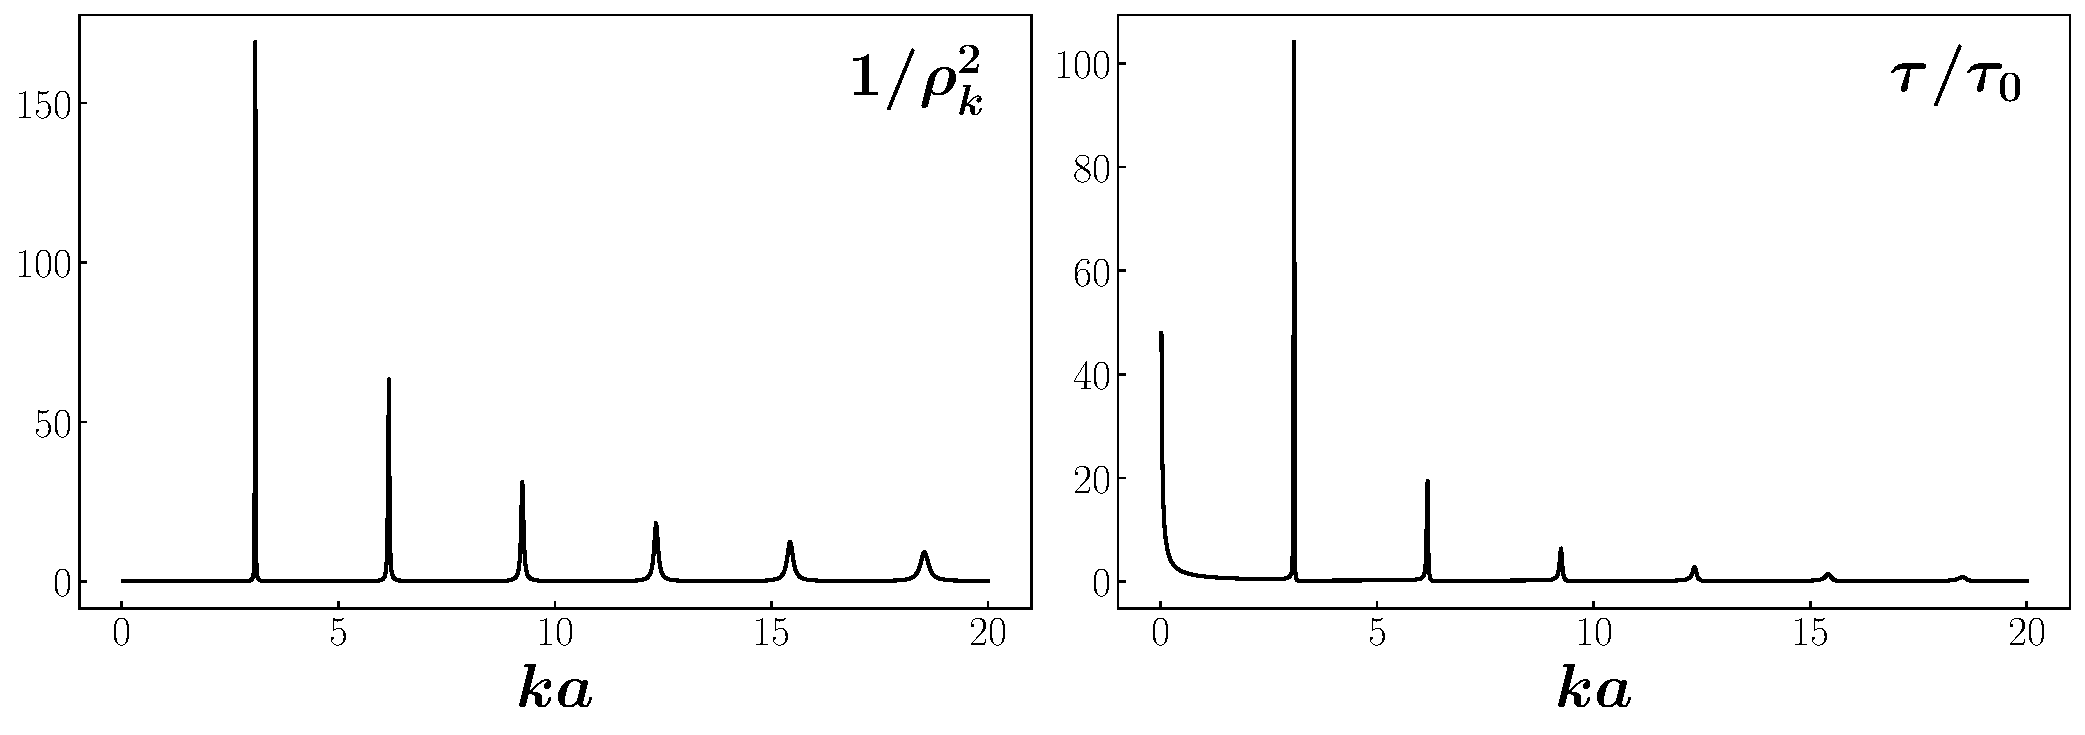
\includegraphics[width=\textwidth]{prob4.pdf}
    \caption{\textbf{Left}: Plot of $1/\rho_{k}^2$ and \textbf{Right}: plot of $\tau/\tau_0$ as functions of $x = ka$ at $x_0 = v_0a = 50$.}
    \label{fig:prob4}
\end{figure}



}


\end{document}
